%%%%%%%%%%%%%%%%%%%%%%% file template.tex %%%%%%%%%%%%%%%%%%%%%%%%%
%
% This is a general template file for the LaTeX package SVJour3
% for Springer journals.          Springer Heidelberg 2010/09/16
%
% Copy it to a new file with a new name and use it as the basis
% for your article. Delete % signs as needed.
%
% This template includes a few options for different layouts and
% content for various journals. Please consult a previous issue of
% your journal as needed.
%
%%%%%%%%%%%%%%%%%%%%%%%%%%%%%%%%%%%%%%%%%%%%%%%%%%%%%%%%%%%%%%%%%%%
%
% First comes an example EPS file -- just ignore it and
% proceed on the \documentclass line
% your LaTeX will extract the file if required
\begin{filecontents*}{example.eps}
%!PS-Adobe-3.0 EPSF-3.0
%%BoundingBox: 19 19 221 221
%%CreationDate: Mon Sep 29 1997
%%Creator: programmed by hand (JK)
%%EndComments
gsave
newpath
  20 20 moveto
  20 220 lineto
  220 220 lineto
  220 20 lineto
closepath
2 setlinewidth
gsave
  .4 setgray fill
grestore
stroke
grestore
\end{filecontents*}
%
\RequirePackage{fix-cm}
%
%\documentclass{svjour3}                     % onecolumn (standard format)
%\documentclass[smallcondensed]{svjour3}     % onecolumn (ditto)
\documentclass[smallextended]{svjour3}       % onecolumn (second format)
%\documentclass[twocolumn]{svjour3}          % twocolumn
%
\smartqed  % flush right qed marks, e.g. at end of proof
%
\usepackage{graphicx}
%
% \usepackage{mathptmx}      % use Times fonts if available on your TeX system
%
% insert here the call for the packages your document requires
%\usepackage{latexsym}
% etc.
%
% please place your own definitions here and don't use \def but
% \newcommand{}{}
%
% Insert the name of "your journal" with
% \journalname{myjournal}
%
\begin{document}

\title{Low-complexity, Sub-band DPD with Sequential Learning%\thanks{Grants or other notes
%about the article that should go on the front page should be
%placed here. General acknowledgments should be placed at the end of the article.}
}
\subtitle{Novel Algorithms and \textsc{Warp}Lab Implementation}

%\titlerunning{Short form of title}        % if too long for running head

\author{Chance Tarver         \and
        Mahmoud Abdelaziz \and
        Lauri Anttila \and
        Mikko Valkama \and
        Joseph~R.~Cavallaro
}

%\authorrunning{Short form of author list} % if too long for running head

\institute{Chance Tarver and Joseph R. Cavallaro \at
	Department of Electrical and Computer Engineering\\
	Rice University, Houston, TX, 77005, USA\\
	\email{\{cat12,cavallar\}@rice.edu}           %  \\
	%             \emph{Present address:} of F. Author  %  if needed
	\and
	Mahmoud Abdelaziz, Lauri Anttila and Mikko Valkama \at
	Department of Electronics and Communication Engineering\\
	Tampere University of Technology, Finland
}


\date{Received: date / Accepted: date}
% The correct dates will be entered by the editor

\maketitle

%Need to revise to include update.
%Current number of words: 138. 
%Recommended: 150 to 250 word
\begin{abstract}
Digital predistortion (DPD) is an effective way of mitigating spurious emission violations without the need of a significant power reduction in the transmitter, thus providing better power efficiency and network coverage. In this paper an iterative version of the IM3 sub-band DPD, proposed earlier by the authors, is presented. The DPD learning is iterated between the higher and lower IM3 sub-bands until a satisfactory performance is achieved for both of them. A sequential DPD learning procedure is also presented in order to reduce the hardware complexity when higher order nonlinearities are incorporated in the DPD learning. Improvements on the convergence speed of the adaptive DPD learning are also achieved via incorporating a variable learning rate and training from previous values. A \textsc{Warp}Lab implementation of the proposed DPD is also shown with excellent suppression of the targeted spurious emissions. 
\keywords{Adaptive filters \and carrier aggregation \and digital predistortion \and nonlinear distortion \and power amplifier \and software-defined radio \and spectrally-agile radio \and spurious emission. }
% \PACS{PACS code1 \and PACS code2 \and more}
% \subclass{MSC code1 \and MSC code2 \and more}
\end{abstract}

\section{Introduction}
\label{intro}
Your text comes here. Separate text sections with
\section{Section title}
\label{sec:1}
Text with citations \cite{RefB} and \cite{RefJ}.
\subsection{Subsection title}
\label{sec:2}
as required. Don't forget to give each section
and subsection a unique label (see Sect.~\ref{sec:1}).
\paragraph{Paragraph headings} Use paragraph headings as needed.
\begin{equation}
a^2+b^2=c^2
\end{equation}

% For one-column wide figures use
\begin{figure}
% Use the relevant command to insert your figure file.
% For example, with the graphicx package use
  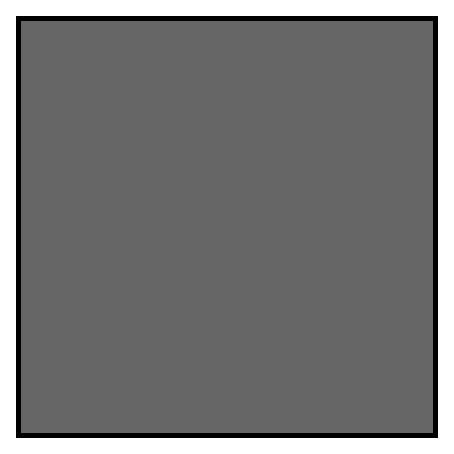
\includegraphics{example.eps}
% figure caption is below the figure
\caption{Please write your figure caption here}
\label{fig:1}       % Give a unique label
\end{figure}
%
% For two-column wide figures use
\begin{figure*}
% Use the relevant command to insert your figure file.
% For example, with the graphicx package use
  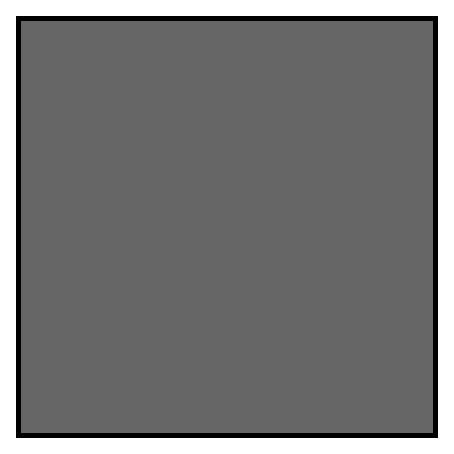
\includegraphics[width=0.75\textwidth]{example.eps}
% figure caption is below the figure
\caption{Please write your figure caption here}
\label{fig:2}       % Give a unique label
\end{figure*}
%
% For tables use
\begin{table}
% table caption is above the table
\caption{Please write your table caption here}
\label{tab:1}       % Give a unique label
% For LaTeX tables use
\begin{tabular}{lll}
\hline\noalign{\smallskip}
first & second & third  \\
\noalign{\smallskip}\hline\noalign{\smallskip}
number & number & number \\
number & number & number \\
\noalign{\smallskip}\hline
\end{tabular}
\end{table}


%\begin{acknowledgements}
%If you'd like to thank anyone, place your comments here
%and remove the percent signs.
%\end{acknowledgements}

% BibTeX users please use one of
%\bibliographystyle{spbasic}      % basic style, author-year citations
%\bibliographystyle{spmpsci}      % mathematics and physical sciences
%\bibliographystyle{spphys}       % APS-like style for physics
%\bibliography{}   % name your BibTeX data base

% Non-BibTeX users please use
\begin{thebibliography}{}
%
% and use \bibitem to create references. Consult the Instructions
% for authors for reference list style.
%
\bibitem{RefJ}
% Format for Journal Reference
Author, Article title, Journal, Volume, page numbers (year)
% Format for books
\bibitem{RefB}
Author, Book title, page numbers. Publisher, place (year)
% etc
\end{thebibliography}

\end{document}
% end of file template.tex

